\chapter{The Southern C-BASS System}
C-BASS uses cassegrain optics- We did not know the shape of the primary reflector and needed to establish this.

\section{System Diagram}
  \subsection{Self-generated RFI considerations}
  \subsection{Remote Operations}

\section{Servo Control}

  \subsection{Description}

    \subsubsection{Requirements}
    \subsubsection{Hardware}
    \subsubsection{Software Integration}

  \subsubsection{Sensor Hardware Design}


    \subsubsection{Optical Pointing}


\section{Primary Dish Profile}
  \subsection{Photogrammetry}
\label{sec:photogrammetry}
Close range photogrammetry is a fairly recent innovation, which allows highly accurate measurements of large objects to be made in an fast, often automated fashion \cite{Luhmann2010}. Photographs are taken from different angles of targets placed in convenient positions on the object being measured. A few of the targets are geometrically coded (see \fign{fig:photogrammetryExampleOfPhotograph}), to ease the orientation of multiple photographs in post-processing . The positions of the individual targets can then be determined, with the accuracy varying as a function of camera resolution, target contrast, and separation angle. Accuracies of up to 1:250 000 are routinely quoted when using carefully calibrated equipment.  Fortunately,  the technique is suitable for use with high end consumer grade cameras \cite{Deng2001}, althought the expected accuracy is lowered.

We made use of this technique in order to characterise the donated Telkom dish.

\subsubsection{Target Choice}

The industry standard is to use retroflective targets. These generally take the form of black adhesive 'stickers' with reflective sections hand pasted into place. These can be expensive to manufacture and put into position.

In the name of completeness and frugality, we also experimented with a slightly unconventional approach, by projecting a series of targets onto the dish surface from a data projector. As can be seen in \fign{fig:photogrammetryExampleOfPhotograph}, this allows a higher density distribution of points across the surface, and is significantly less expensive and time consuming to implement. 

However this technique suffers from a few obvious limitations, namely resolution and contrast. By fitting centroids to a target position, photogrammetry routinely achieves sub-pixel resolution in the point's position. Poor resolution and low contrast adversely effect this process, to such and extent that we were unable to get a well constrained solution using the projected targets, and after many less than glamourous nights, decided to use the industry standard retroreflective targets. 


\begin{figure}[ht]
 \centering
 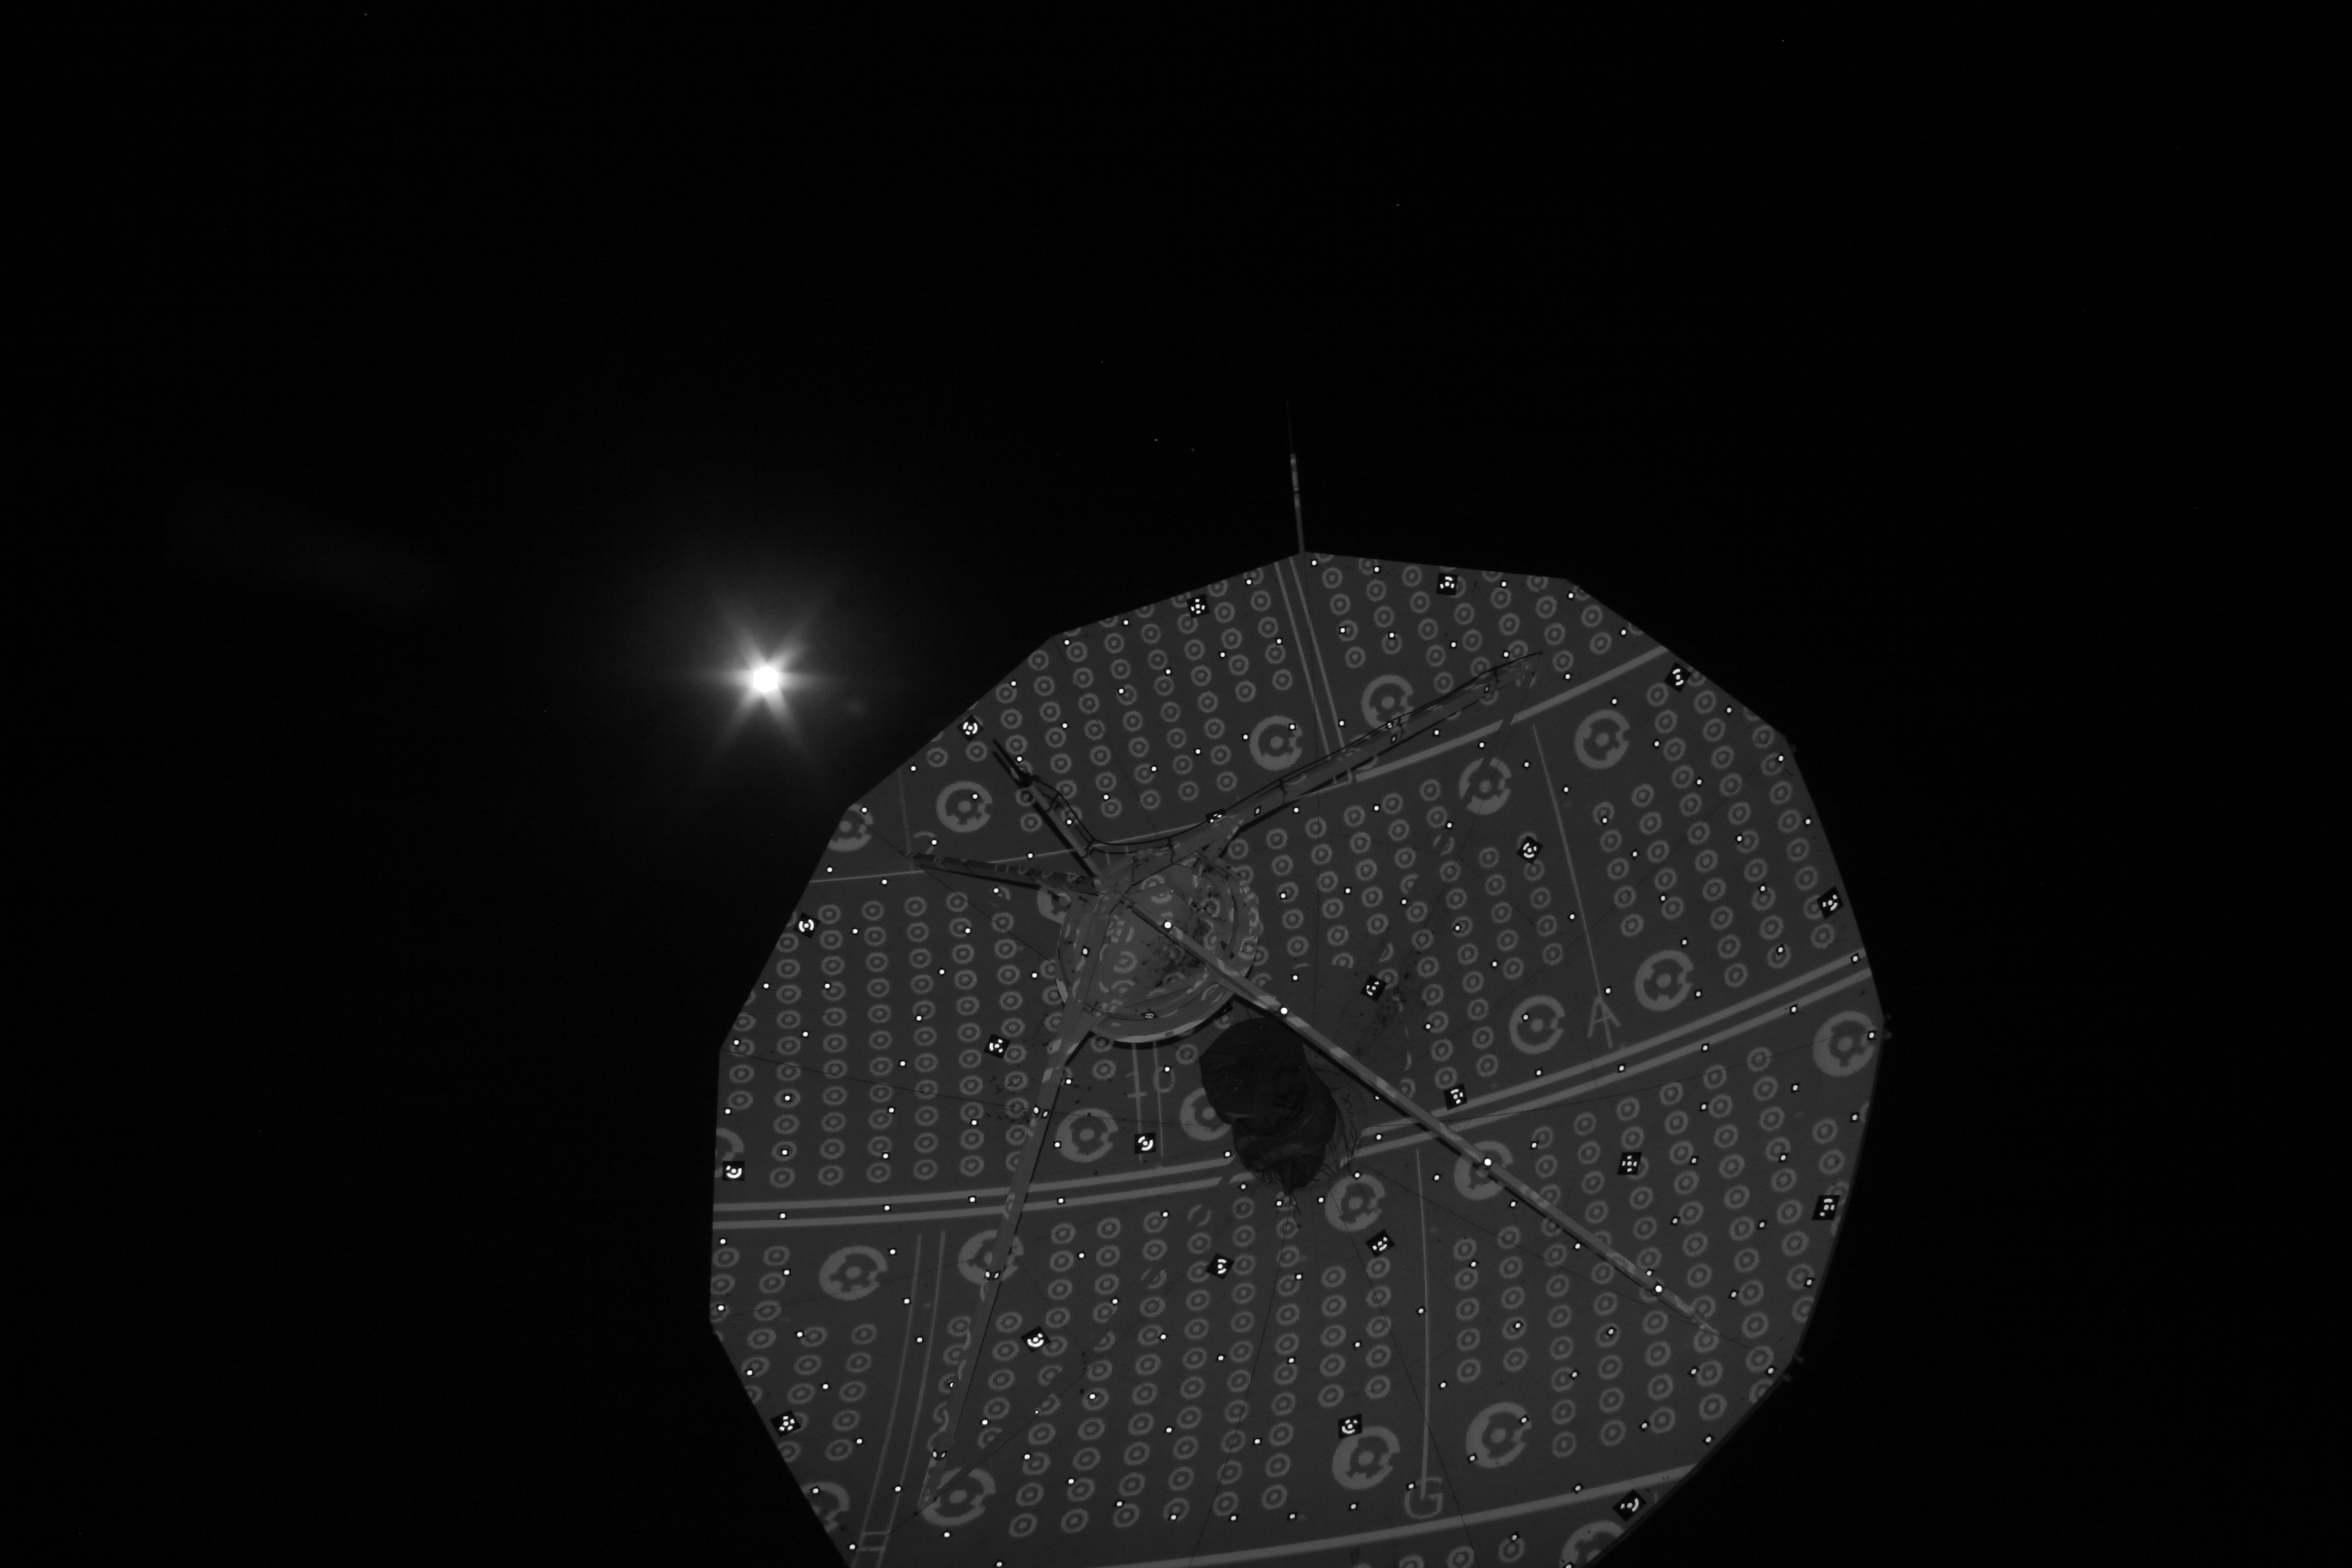
\includegraphics[width=\textwidth]{./images/photogrammetry/PhotoExamples/projectedAndRetrofelctive.JPG}
 % projectedAndRetrofelctive.JPG: 3504x2336 pixel, 72dpi, 123.61x82.41 cm, bb=
 \caption{An example of a photograph taken of the dish surface. The high contrast, bright points are retroflective targets, while the other (more densely distributed) points were projected onto the dish from a data projector. The targets consist of both standard circular targets, and geometrically coded targets to help in the post-processing photograph orientation.}
 \label{fig:photogrammetryExampleOfPhotograph}
\end{figure}

\subsubsection{Primary Shape}
The primary surface is not a 'strict' paraboloid, but rather falls into the category of 'shaped optics'. This type of design features an offset from the traditional parabolic reflector described in detail in \citeasnoun{Galindo1964}, and is a technique used to optimise the aperture efficiency of antennas.

\begin{figure}
 \centering
 \subfloat[Section through the dish surface relative to best fit parabola]{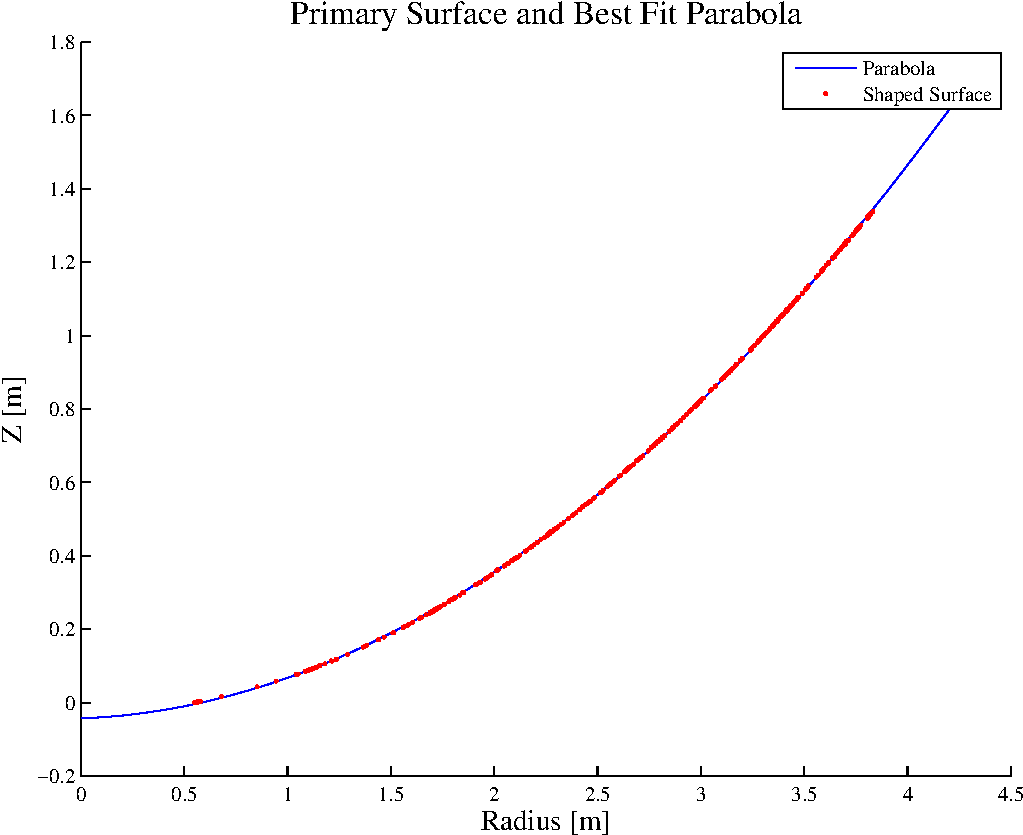
\includegraphics[width=0.4\textwidth,height=0.25\textheight]{images/photogrammetry/section.pdf}}
\hspace{0.2cm}
 \subfloat[Exaggerated (x20) section difference from the best fit parabola to show the shaping of the primary]{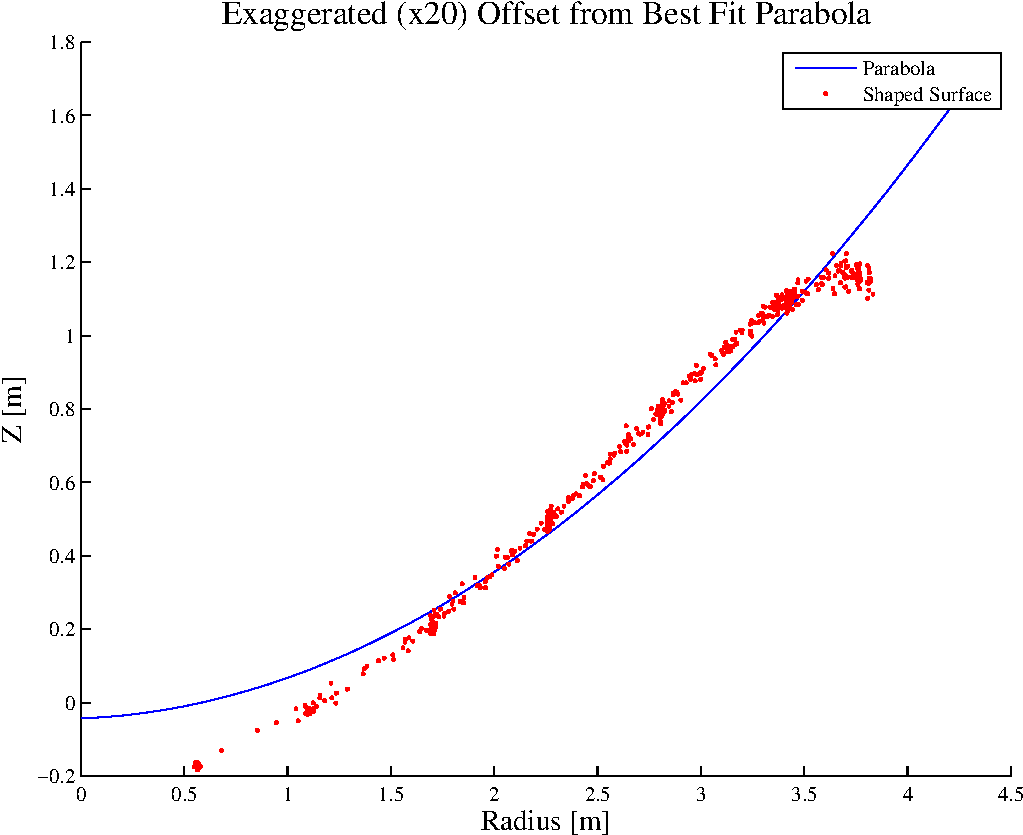
\includegraphics[width=0.4\textwidth,height=0.25\textheight]{images/photogrammetry/offset_section.pdf}}\\
 %\subfloat[Colour shows deviation from best-fit parabola when viewing the dish face on]{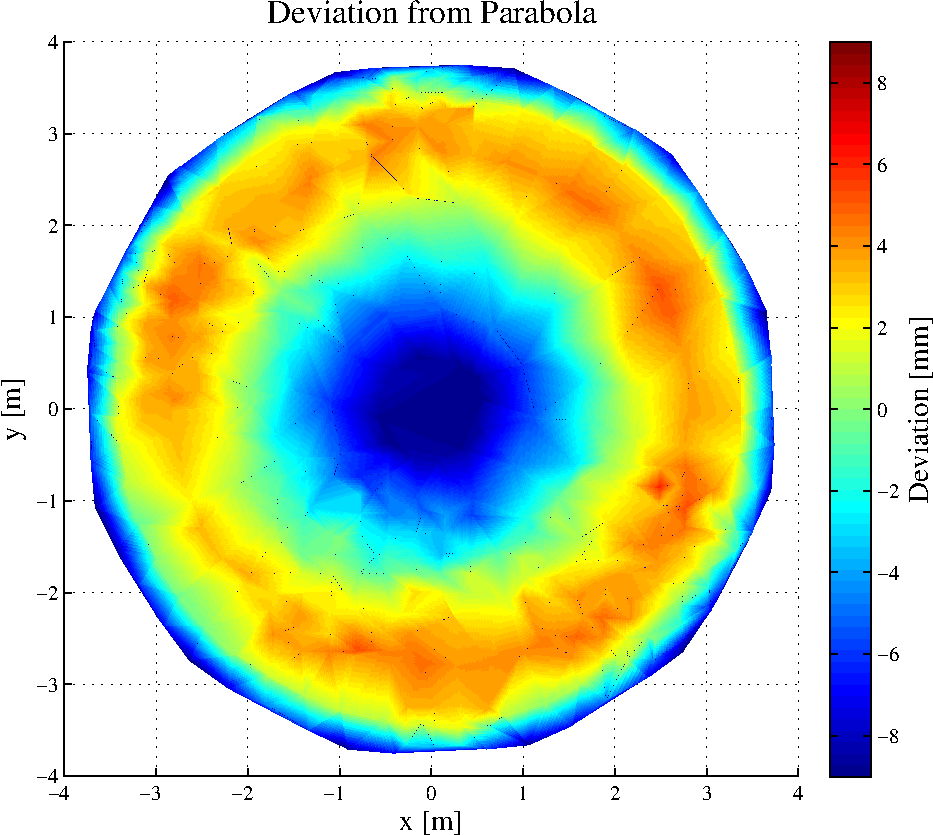
\includegraphics[width=0.4\textwidth,height=0.25\textheight]{images/photogrammetry/shape.pdf}}\\
 \subfloat[Colour shows the deviation from model used in optical design before transport- RMS=1.61~mm ]{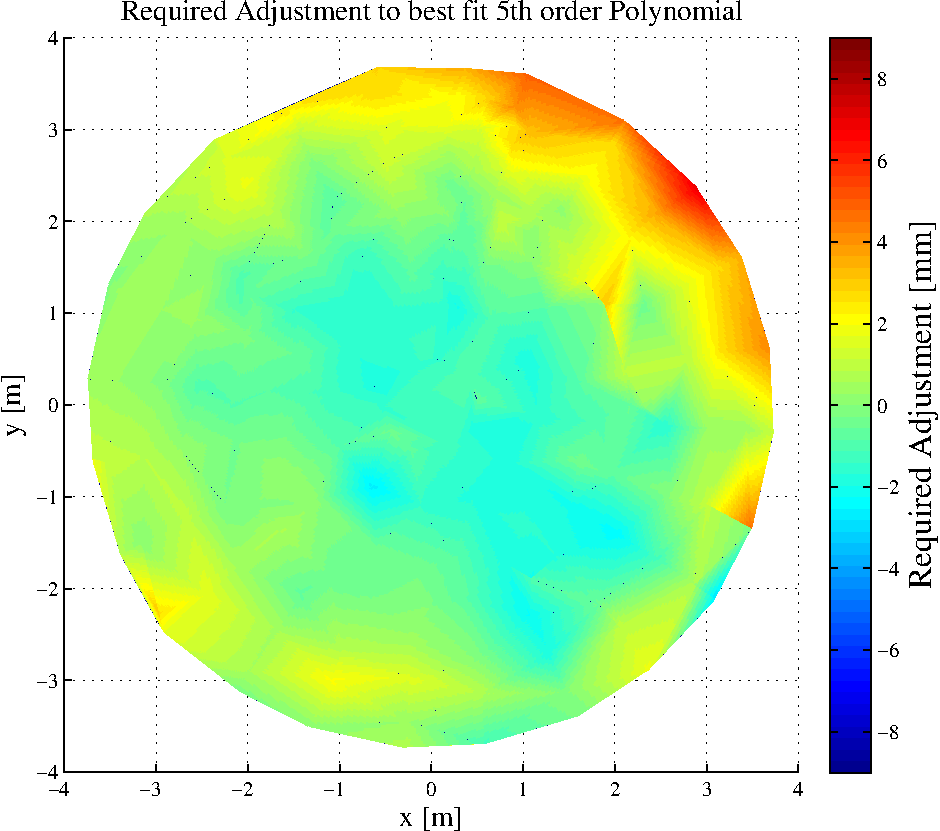
\includegraphics[width=0.4\textwidth,height=0.25\textheight]{images/photogrammetry/before.pdf}\label{fig:before_transport}}
\hspace{0.2cm} 
\subfloat[Colour shows the deviation from model used in optical design after transport- RMS=3.91~mm ]{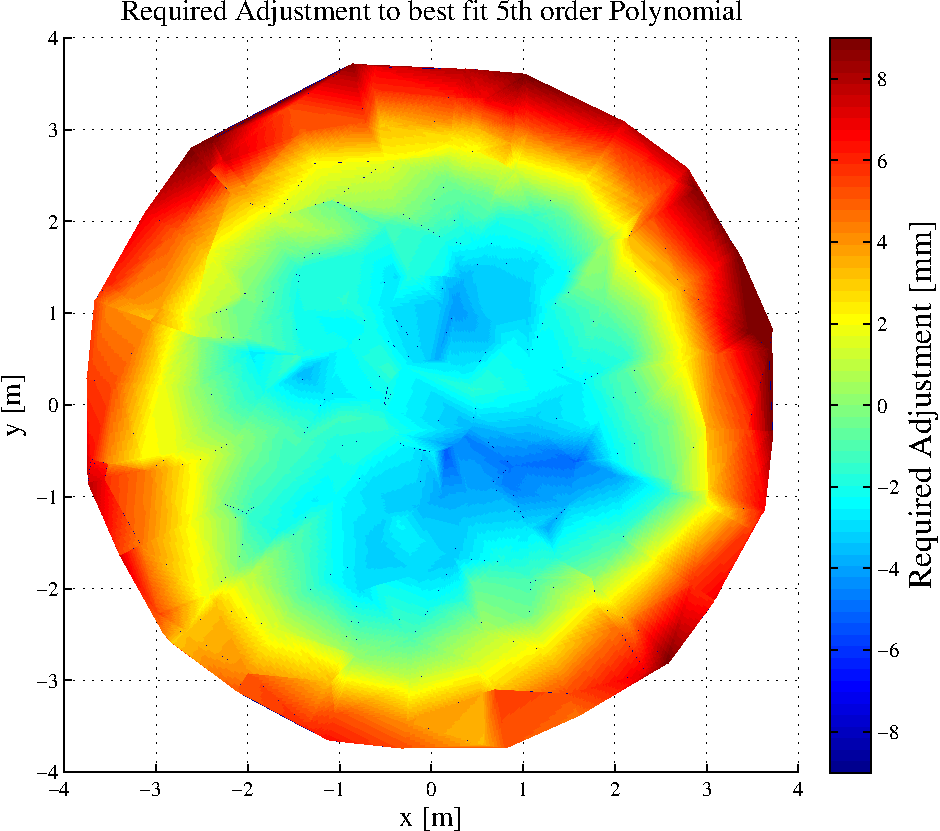
\includegraphics[width=0.4\textwidth,height=0.25\textheight]{images/photogrammetry/after.pdf}\label{fig:after_transport}}
 % newdish_upgrade.jpg: 1280x728 pixel, 72dpi, 45.16x25.68 cm, bb=
 \caption{Primary reflector offsets from design goal obtained from photogrammetric measurements of the South African 7.6~m dish. The primary shape used in the optical design is a 5th order polynomial fitted to the shape in (a) and (b). The offsets shown in (c) and (d) are with respect to this 5th order polynomial.}
 \label{fig:dish_surface}
\end{figure}



    \subsubsection{Transportation Quality Control}

\subsubsection{Independent Check of Photogrammetry and First Light}
\label{sec:first_light}
We used a modified 12~GHz receiver and custom designed rectangular feed horn \cite{meeks_1976} to observe powerful Ku Band Geostationary Satellites. A photograph of the assembled receiver is included in \fign{fig:feed}. It is possible to establish a focal point by scanning through a source and adjusting the position of the feed to maximise the observed power. At the position of maximum received power, the phase centre of the feed and the focal point of the antenna are coincident, providing a direct measurement of the antenna focal point. The results of this experiment are shown in \fign{fig:focal_point}. It is also possible (using ray tracing) to derive an expected focal point given the photogrammetric shape described in Section~\ref{sec:photogrammetry}. Comparing the measured and expected focal points (derived using the \textit{GRASP8} ray tracing software package), provides an independent check on the quality of the photogrammetry results.  

 The consistency between expected and measured focal point was very reassuring and confirmed our photogrammetry data. A diagram of the optical layout of the antenna is \fign{fig:optics}

\begin{figure}[ht]
 \centering
 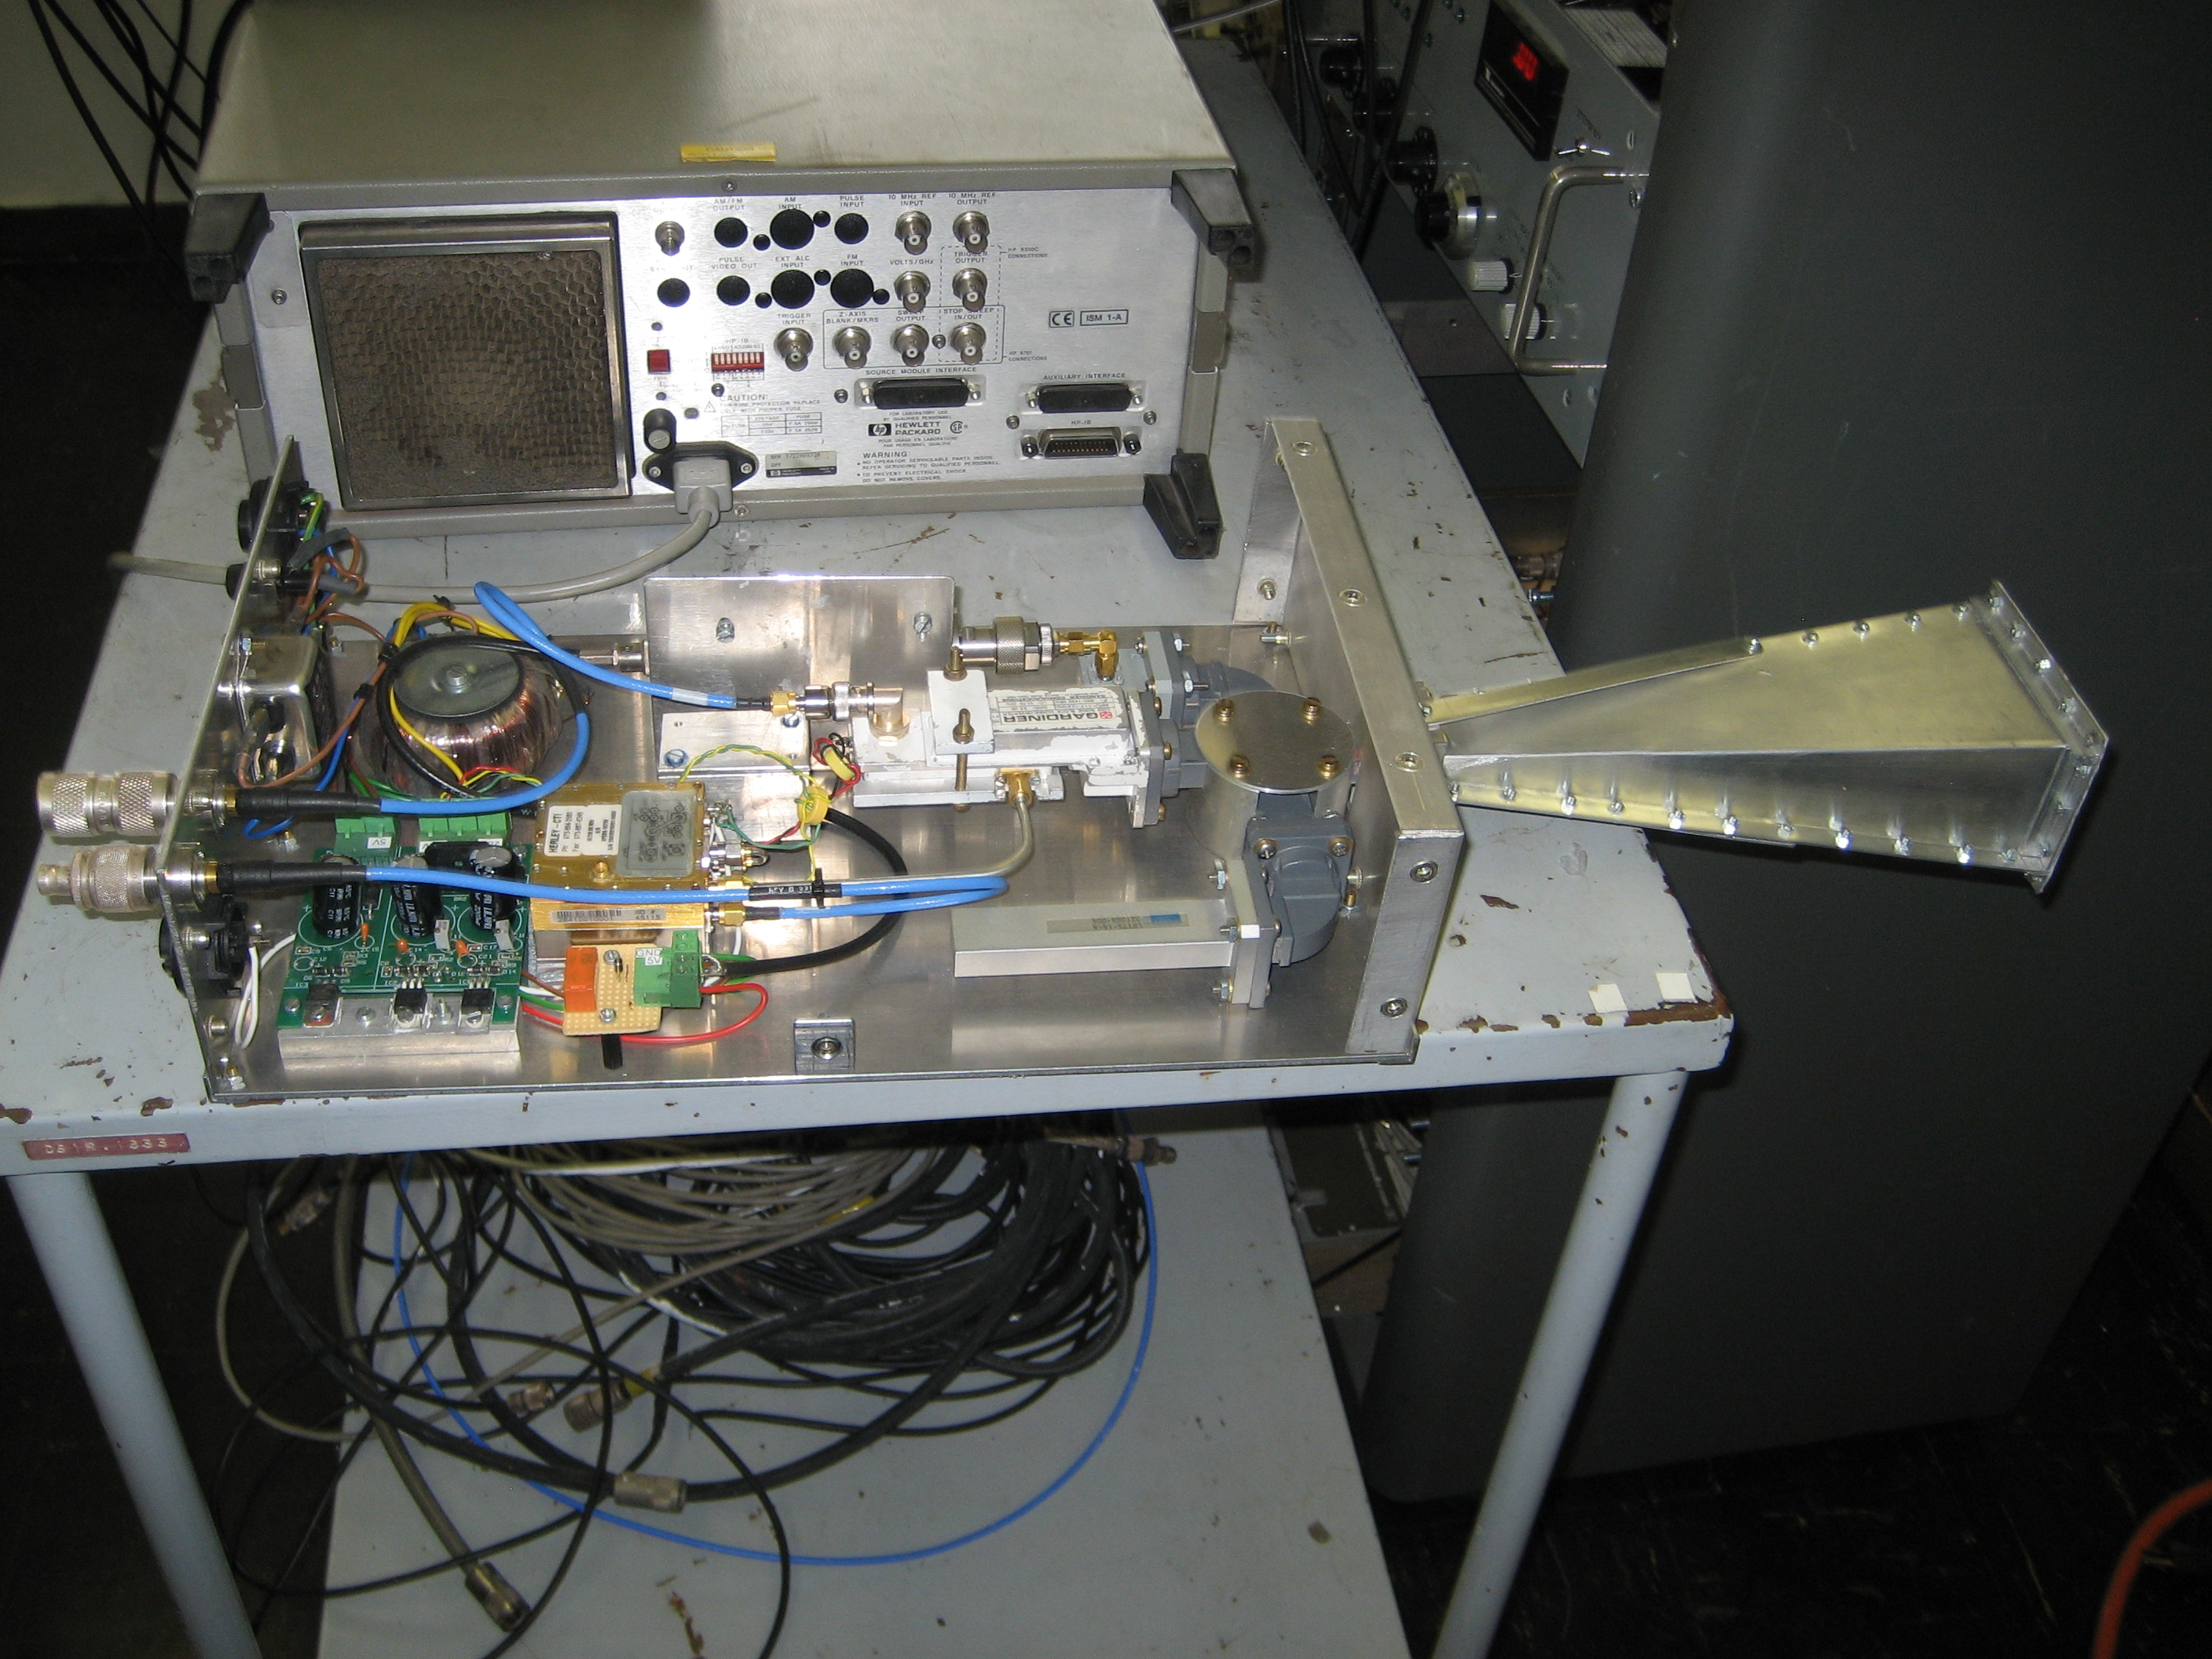
\includegraphics[width=\textwidth]{images/PAS7_cross_scans/img_1093.jpg}
 % img_1093.jpg: 2816x2112 pixel, 180dpi, 39.74x29.80 cm, bb=
 \caption{12~GHz Receiver and newly designed feed}
 \label{fig:feed}
\end{figure}

\begin{figure}[ht]
 \centering
 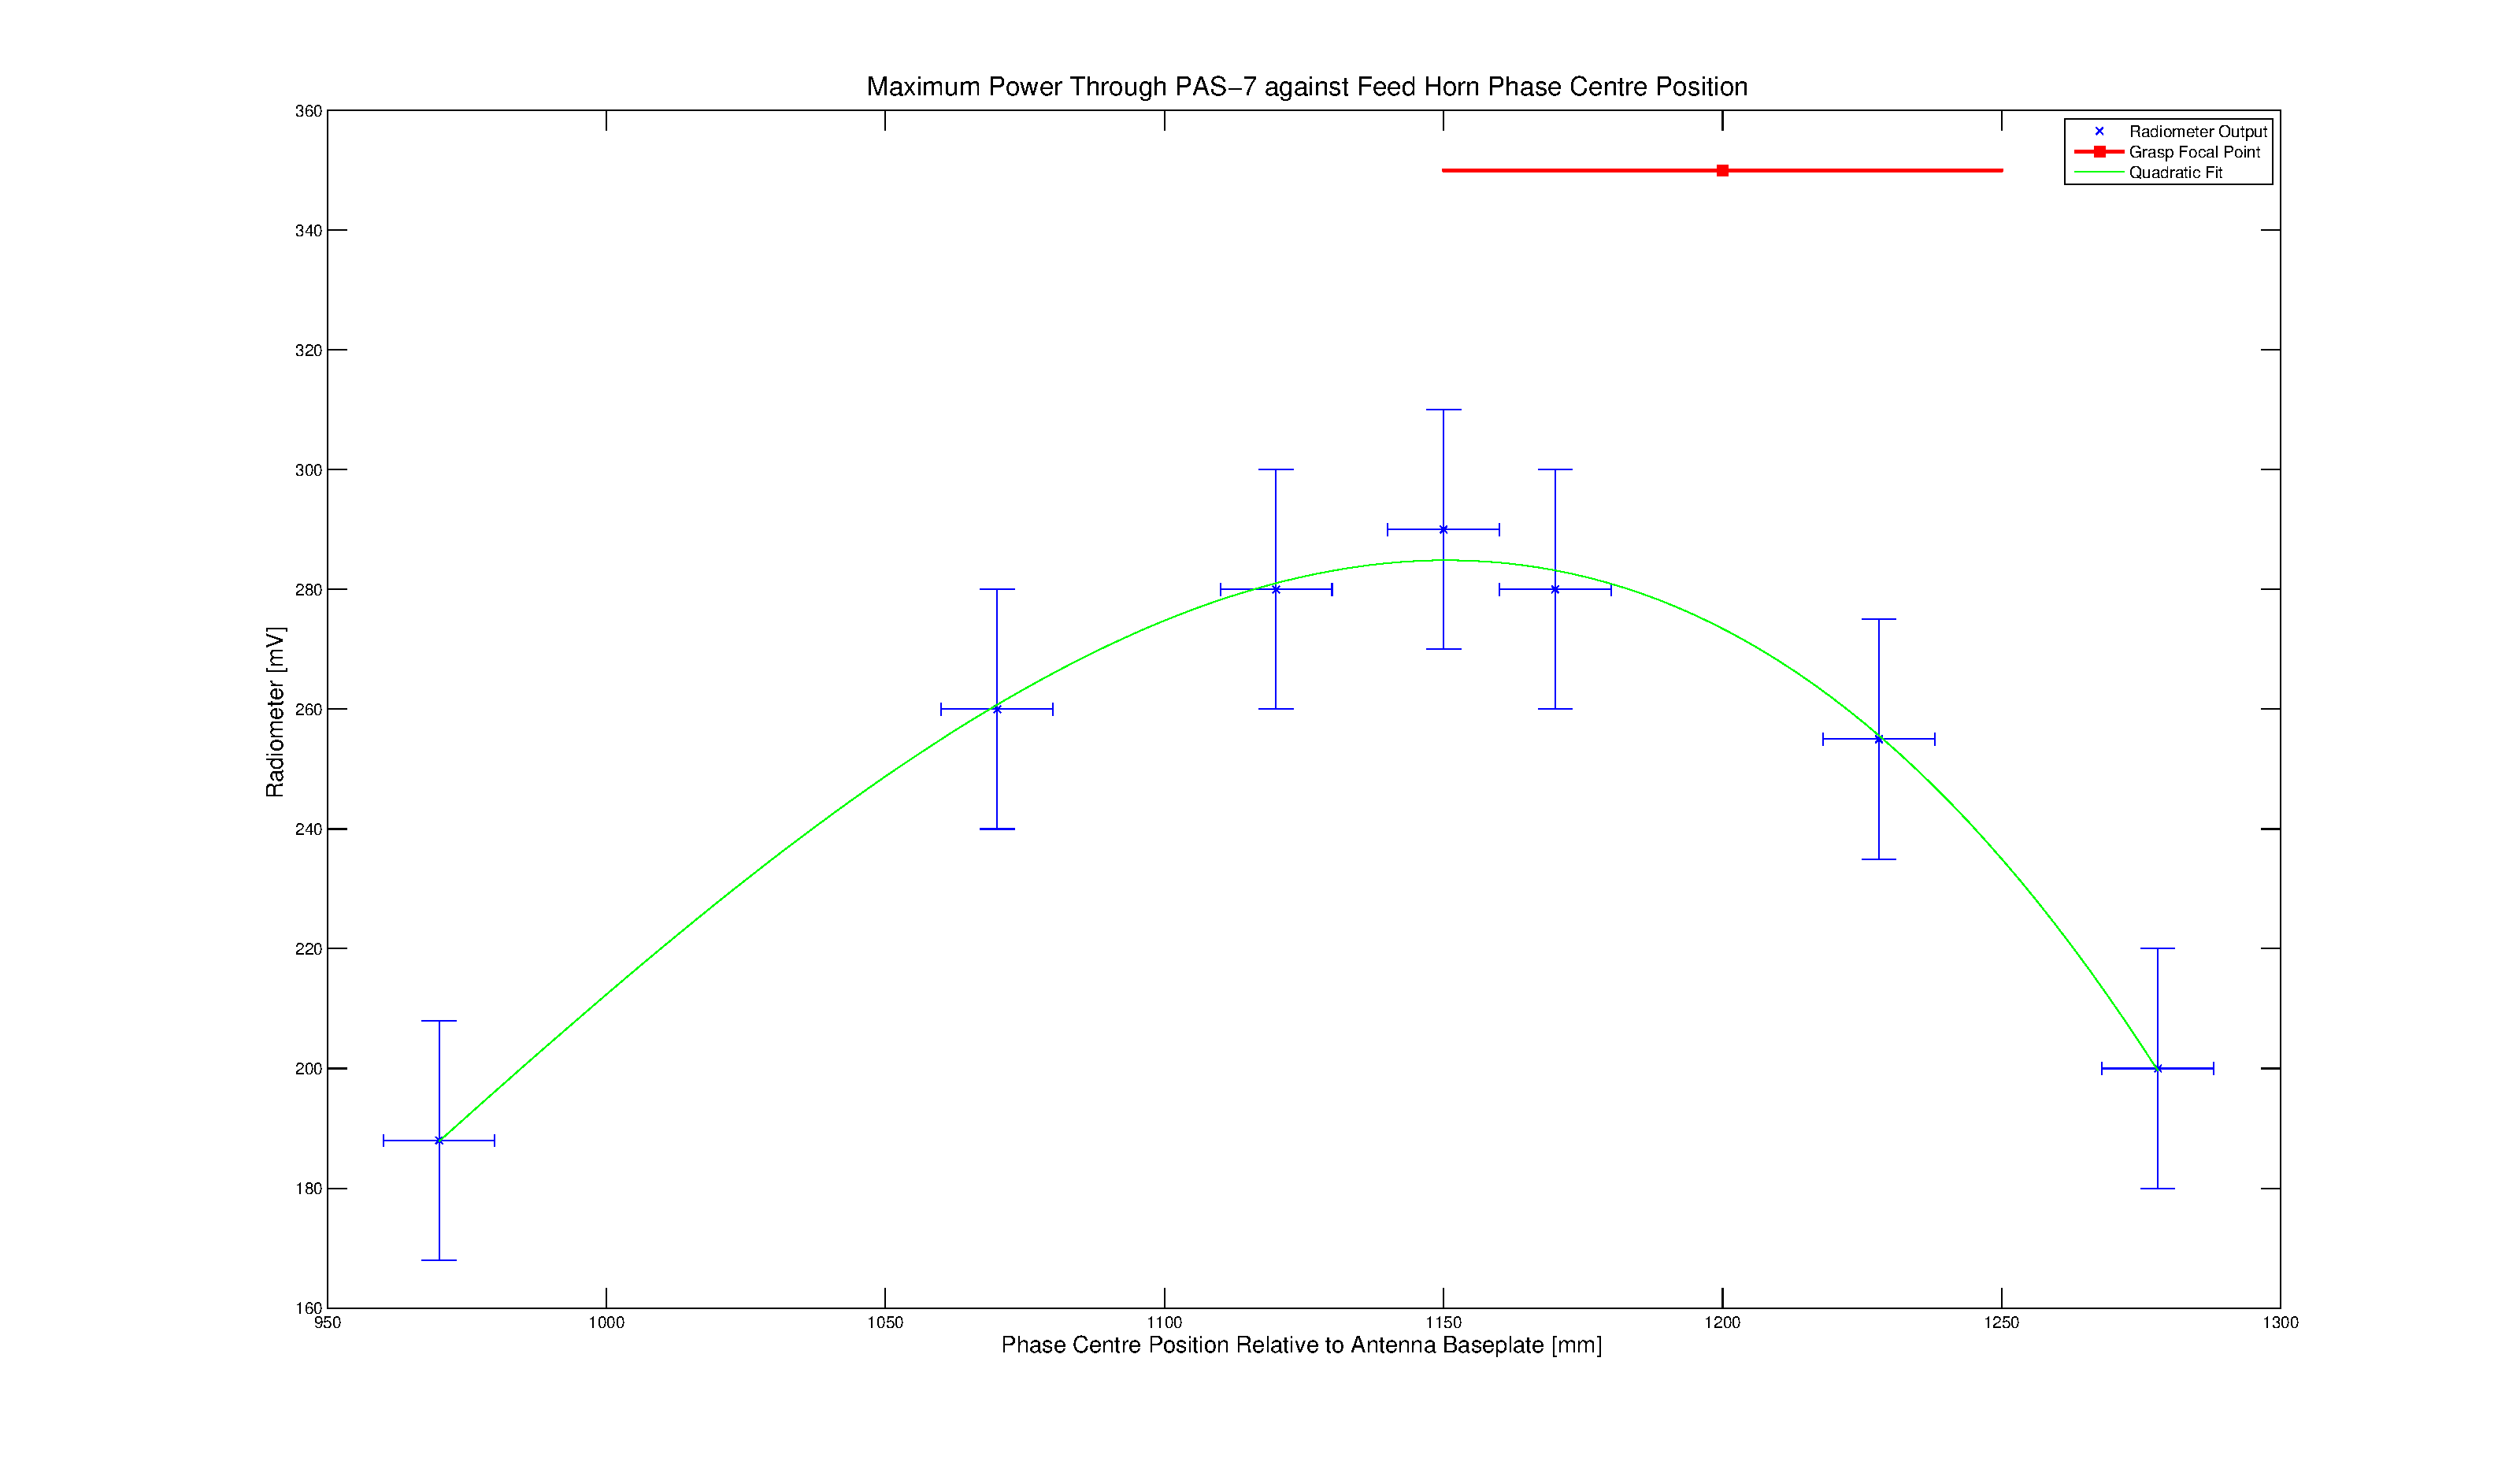
\includegraphics[width=\textwidth]{images/PAS7_cross_scans/focal_point.pdf}
 % focal_point.png: 1920x1076 pixel, 90dpi, 54.19x30.37 cm, bb=0 0 1536 861
 \caption{Maximum radiometer output voltage (which is proportional to RF power) when scanning through PAS-7, is plotted against feed phase centre position during the scan. The red marker shows the Grasp Software package prediction of the antenna focal point (1200$\pm$50~mm), calculated using the photogrammetry data of the primary and secondary reflector surface shapes. Maximum received power is expected when the feed phase centre and antenna focal point are coincident. The measurements show a maximum power at a feed phase centre position of $\approx$1150mm, which is (just) within the uncertainty of the Grasp simulation prediction of the antenna focal point (1200$\pm$50mm). Since the Grasp focal point is calculated using the photogrammetry data, this provides an independent 'sanity' check of the measurements used to design the new optics of the C-BASS antenna.}
 \label{fig:focal_point}
\end{figure}

\begin{figure}[ht]
 \centering
 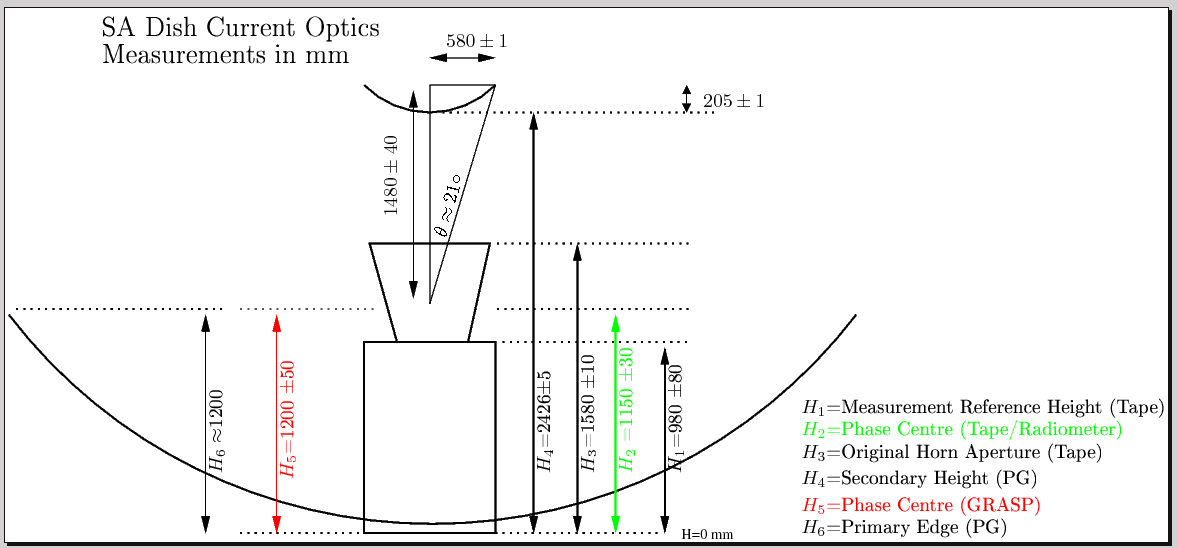
\includegraphics[width=\textwidth]{images/optics/optics4_after.png}
 % optics4_after.png: 1178x548 pixel, 98dpi, 30.53x14.20 cm, bb=
 \caption{Optics of the system before modifications- estimated uncertainties are approximate and not rigorously derived. Note this is the optical configuration prior to the redesign of the optics for the C-BASS experiment. These measurements are confirmed by both photogrammetry and the focal point check described in Section~\ref{sec:first_light}}
 \label{fig:optics}
\end{figure}




\section{Site Establishment}
\subsection{Infrastructure}
  \subsubsection{Power Provision}
  \subsubsection{Optical Fibre}
  \subsubsection{Access}
    \subsubsection{Control Shelter Considerations}
    \subsubsection{RFI Survey}


\subsection{Science Requirements}
  


